\ifdefined \buildingFullOPALManual \else


%\ifx \@buildingFullOPALManual \@empty
%\else

%\documentclass[12pt,a4paper]{report}
\documentclass[a4paper]{book}

%% does not work in Latex2Html mode
%\usepackage{hyperref}

\usepackage[T1]{fontenc}
\usepackage{url}
\usepackage{html}
\usepackage{epic}
\usepackage{eepic}
\usepackage{makeidx}
\usepackage{array}
\usepackage{times}
\usepackage{amsmath}
\usepackage{amsxtra}
\usepackage{bm}
\usepackage[thin,thinp,thinc]{esdiff}
\usepackage{graphicx}
\usepackage{dingbat}
\usepackage{color}
\usepackage{subfig}
\usepackage{boxedminipage}
\usepackage{alltt}
\usepackage{nicefrac}
\usepackage{calc}
%\usepackage{pdfdraftcopy}             % Draft
\usepackage{tikz}
\usetikzlibrary{
  er,3d,calc,fadings,trees,positioning,arrows,chains,decorations.pathreplacing,
  decorations.pathmorphing,shapes,shapes.symbols,shapes.arrows,matrix,through,decorations.text
}

\tikzset{
  >=stealth',
  punktchain/.style={rectangle,rounded corners, draw=black, very thick,text width=10em,
                     minimum height=3em, text centered, on chain},
  line/.style={draw, thick, <-},
  element/.style={tape,top color=white,bottom color=blue!50!black!60!,minimum width=8em,
                  draw=blue!40!black!90, very thick,text width=10em, minimum height=3.5em,
                  text centered, on chain},
  every join/.style={->, thick,shorten >=1pt},
  tuborg/.style={decorate},
  tubnode/.style={midway, right=2pt}
}

\tikzstyle{material}=[draw, fill=blue!20, text width=16.0em, text centered, minimum height=1.5em]
\tikzstyle{diagramstep} = [material, text width=20em, minimum width=10em, minimum height=3em, rounded corners]
\tikzstyle{line} = [draw, thick, color=black!50, -latex']

\usepackage{booktabs}
\usepackage{xspace}
\usepackage{xstring}

\usepackage{fancyvrb}
\usepackage{rotating}
\usepackage{float}

\usepackage{tabularx}
\usepackage{longtable}
\setcounter{LTchunksize}{3}

\usepackage[section]{placeins}
\usepackage{MnSymbol}
\usepackage{microtype}
\usepackage{setspace}
\usepackage{dcolumn}

\usepackage[vmargin={3.0cm,3.0cm},
            hmargin={2.0cm,3.0cm}]{geometry}

\usepackage{upgreek}
\usepackage[binary-units=true]{siunitx}
\sisetup{exponent-product = \cdot,math-ohm=\Upomega,text-ohm=\ensuremath{\Upomega}}
\DeclareSIUnit{\clight}{c}
\DeclareSIUnit\gauss{Ga}

\usepackage{engord}
\usepackage{wasysym}
\DeclareSIUnit[number-unit-product = \,]{\permill}{\permil}

\usepackage{hyperref}
\hypersetup{
    pdftitle          = The OPAL Framework,
    pdfauthor         = {Andreas Adelmann, Achim Gsell, Valeria Rizzoglio, Christof Metzger-Kraus,
                         Yves Ineichen, Xiaoying Pang, Steve Russell, Chuan Wang, Jianjun Yang,
                         Suzanne Sheehy, Chris Rogers, Daniel Winklehner},
    pdfsubject        = User's Reference Manual,
    pdffitwindow      = true,               % page fit to window when opened
    pdfnewwindow      = true,               % links in new window
    colorlinks        = true,               % false: boxed links; true: colored links
    linkcolor         = black!80!green,     % color of internal links
    citecolor         = black!20!red,       % color of links to bibliography
    urlcolor          = blue,               % color of external links
    breaklinks        = true,
    bookmarksnumbered = true,
    plainpages        = false
}

\usepackage{ifthen}

\newif \iflinuxwindows
\linuxwindowstrue   % set this to true when building the manual on Linux or Windows
\iflinuxwindows
\usepackage{epstopdf}
\fi

\usepackage[backend=biber,
            style=phys,
            biblabel=brackets,
            maxnames=3,
            doi=true,
            isbn=true,
            url=true]{biblatex}
%---- macros ----

\renewcommand{\topfraction}{1.0}
\renewcommand{\bottomfraction}{1.0}
\renewcommand{\textfraction}{0.0}
\renewcommand{\arraystretch}{2.0}
\newenvironment{tex2html_nowrap}{}{}


\newcommand{\Newline}{\hfil \\}


\newsavebox{\ExampleBox}
\newenvironment{example}
 {\VerbatimEnvironment
  \begin{flushleft}
  \begin{lrbox}{\ExampleBox}
    \begin{minipage}{\linewidth}
  \begin{Verbatim}[frame=lines,xleftmargin=0cm,fontsize=\footnotesize,samepage=true]}
 {\end{Verbatim}
  \end{minipage}
  \end{lrbox}
  \mbox{\usebox{\ExampleBox}}
  \end{flushleft}
 }

\newenvironment{longexample}
{\Verbatim[frame=lines,xleftmargin=0mm,fontsize=\footnotesize]}
{\endVerbatim}

%\examplefromfile{filename} reads in a text file and displays it in the document.
\newcommand{\examplefromfile}[1]{
\VerbatimInput[frame=lines,xleftmargin=0mm,fontsize=\footnotesize,label=\texttt{#1}]{#1}}

%for upright d of differentials
\makeatletter
\newcount\my@repeat@count

\newcommand{\myrepeat}[2]{%
  \begingroup
  \my@repeat@count=\z@
  \@whilenum\my@repeat@count<#1\do{#2\advance\my@repeat@count\@ne}%
  \endgroup
}

\newcommand{\differential}[1]{\ifstrempty{#1}{\ES@dop\ES@difint}{\ES@dop^{#1}\ES@difint}}
\newcommand{\pdifferential}[1]{\ifstrempty{#1}{{\partial\,}}{{\partial^{#1}\,}}}

\makeatother

\newcommand{\der}[3][]{\frac{\differential{#1}#2}{\differential{}\ifstrempty{#1}{#3}{#3^#1}}}
\newcommand{\parder}[3][]{\frac{\pdifferential{#1}#2}{\pdifferential{}\ifstrempty{#1}{#3}{#3^#1}}}
\newcommand{\niceder}[3][]{\nicefrac{\differential{#1}#2}{\differential{}\ifstrempty{#1}{#3}{#3^#1}}}
\newcommand{\uglyder}[3][]{{\differential{#1}#2}/{\differential{}\ifstrempty{#1}{#3}{#3^#1}}}
\newcommand{\uglyparder}[3][]{{\pdifferential{#1}#2}/{\pdifferential{}\ifstrempty{#1}{#3}{#3^#1}}}
\newcommand{\dd}[1][]{\; \differential{#1}}
\newcommand{\primed}{^{\prime}}
\newcommand{\dprimed}{^{\prime\prime}}
\newcommand{\nprimed}[1]{^{\myrepeat{#1}{\prime}}}

%Editing Macros
\newcommand{\TODO}[1]{{\color{red}\ifthenelse{\boolean{ShowDebug}}{[TODO: #1]}{}}}



%text in gray box
\newsavebox{\fmbox}
\definecolor{lightgray}{gray}{0.95}
\newenvironment{fmpage}
   {\vspace{-1.0cm}\begin{lrbox}{\fmbox}\begin{minipage}[t]{13.5cm}\vspace{0.1cm}}
   {\vspace{-0.4cm}\end{minipage}\end{lrbox}\begin{center}\fcolorbox{black}{lightgray}{\usebox{\fmbox}}\end{center}}


% Definition new signes
\newcommand{\R}{{\mathbb R}} % real numbers
\newcommand{\Q}{{\mathbb Q}} % rational numbers
\newcommand{\Z}{{\mathbb Z}} % integer numbers
\newcommand{\N}{{\mathbb N}} % natural numbers

\newcommand{\mad}{\textsc{mad}\xspace}
\newcommand{\madnine}{\textsc{mad9}\xspace}
\newcommand{\madninep}{\textsc{mad9p}\xspace}
\newcommand{\madeight}{\textsc{mad8}\xspace}
\newcommand{\classic}{\textsc{classic}\xspace}

\makeatletter
\newcommand{\opal@impl}{\textsc{Opal}}
\newcommand{\opalt@impl}{\textsc{Opal-t}}
\newcommand{\opalcycl@impl}{\textsc{Opal-cycl}}
\newcommand{\opalmap@impl}{\textsc{Opal-map}}
\newcommand{\opalenv@impl}{\textsc{Opal-e}}

\newcommand{\opal}{\opal@impl\xspace}
\newcommand{\opalt}{\opalt@impl\xspace}
\newcommand{\opalcycl}{\opalcycl@impl\xspace}
\newcommand{\opalmap}{\opalmap@impl\xspace}
\newcommand{\opalenv}{\opalenv@impl\xspace}

\newcommand{\noopalt}{\leftthumbsdown \opalt@impl\xspace}
\newcommand{\noopalcycl}{\leftthumbsdown \opalcycl@impl\xspace}
\newcommand{\noopalmap}{\leftthumbsdown \opalmap@impl\xspace}
\newcommand{\noopalenv}{\leftthumbsdown \opalenv@impl\xspace}
\makeatother

\newcommand{\impactt}{\textsc{Impact-t}\xspace}
\newcommand{\partroot}{\textsc{H5root}}


\newcommand{\latermore}{More details will be given in Version 1.6.0}


\newcommand{\lieop}[1]{{:}{#1}{:}}

\newcommand{\rms}[1]{\overset{\sim}{#1}}

\newcommand{\sprod}{\cdot}
\newcommand{\vprod}{\times}
\newcommand{\matr}[1]{\mathcal{#1}}
\renewcommand{\vec}[1]{{\bm{#1}}}
\newcommand{\transpose}[1]{#1^\intercal}
\renewcommand{\epsilon}{\varepsilon}

\newcommand{\keyword}[2][]{\ifstrempty{#1}{\texttt{\expandafter\MakeUppercase\expandafter{#2}}}{\hyperref[#1]{\texttt{\expandafter\MakeUppercase\expandafter{#2}}}}}
\newcommand{\tabline}[3][]{\keyword[#1]{#2}& #3 \\}
\newcommand{\tabheadcell}[1]{{\bfseries #1}}

\newcommand*\kdescriptionlabel[1]{\hspace\labelsep
                                \normalfont\keyword{#1}\index{#1}}
\makeatletter
\newenvironment{kdescription}
               {\list{}{\labelwidth\z@ \itemindent-\leftmargin
                        \let\makelabel\kdescriptionlabel}}
               {\endlist}
\makeatother

\ExplSyntaxOn
\NewDocumentCommand{\tabhead}{ m }
 {
  \seq_set_split:Nnn \l_tmpa_seq { & } { #1 }
  \bfseries \seq_use:Nn \l_tmpa_seq { & \bfseries } \\
 }

\NewDocumentCommand \multrefImpl { O{ } m m m } {
  \ifnumgreater{\clist_count:n {#4}}{1}{
    \seq_set_from_clist:Nn \l_tmpa_seq { #4 }

    \seq_set_map:NNn \l_tmpb_seq \l_tmpa_seq { \exp_not:n { \ref{#3:##1} } }
    \ifstrempty{#1}{#2s}{#1}~\seq_use:Nnnn \l_tmpb_seq {\ and\ } {,\ } {,\ and\ }
  }{
    #2~\ref{#3:#4}
  }
}

\NewDocumentCommand \multeqnrefImpl { m } {
  \ifnumgreater{\clist_count:n {#1}}{1}{
    \seq_set_from_clist:Nn \l_tmpa_seq { #1 }

    \seq_set_map:NNn \l_tmpb_seq \l_tmpa_seq { \exp_not:n { \eqref{eq:##1} } }
    Equations~\seq_use:Nnnn \l_tmpb_seq {\ and\ } {,\ } {,\ and\ }
  }{
    Equation~\eqref{eq:#1}
  }
}
\ExplSyntaxOff


%Abbreviations for Equations, Figures, and Tables
%\newcommand{\Equation}[1]{Equation~\eqref{#1}}

\newcommand{\bibref}[2]{#1 \cite{bib:#2}}
\newcommand{\figref}[1]{\multrefImpl{Figure}{fig}{#1}}
\newcommand{\chpref}[1]{\multrefImpl{Chapter}{chp}{#1}}
\newcommand{\appref}[1]{\multrefImpl[Appendices]{Appendix}{chp}{#1}}
\newcommand{\secref}[1]{\multrefImpl{Section}{sec}{#1}}
\newcommand{\ssecref}[1]{\multrefImpl{Section}{ssec}{#1}}
\newcommand{\tabref}[1]{\multrefImpl{Table}{tab}{#1}}
\newcommand{\eqnref}[1]{\multeqnrefImpl{#1}}

\newcommand{\seefig}[1]{(see~\figref{#1})}
\newcommand{\seechp}[1]{(see~\chpref{#1})}
\newcommand{\seesec}[1]{(see~\secref{#1})}
\newcommand{\seessec}[1]{(see~\ssecref{#1})}
\newcommand{\seetab}[1]{(see~\tabref{#1})}
\newcommand{\seeeqn}[1]{(see~\eqnref{#1})}

\newcommand{\filename}[1]{\emph{#1}}


% Define distances for bordering
\newcommand{\blockdist}{1.3}
\newcommand{\edgedist}{1.5}
\newcommand{\diagramstep}[2]{node (p#1) [diagramstep] {#2}}


% place chapter title page on odd pages
\let\stdchapter\chapter
\makeatletter
\renewcommand*{\chapter}{\if@openright\cleardoublepage\else\clearpage\fi\stdchapter}

\makeatother

\IfFileExists{./version.tex}{%
  \newcommand{\opalversion}[1]{Version \ifstrempty{#1}{1.9.0}{#1}\xspace}
%
}%
{%
  \newcommand{\opalversion}[1]{\ifstrempty{#1}{current Version}{Version #1}\xspace}%
}
\newboolean{ShowMap}
\setboolean{ShowMap}{false}

\newboolean{ShowEnv}
\setboolean{ShowEnv}{false}

\newboolean{ShowDebug}
\setboolean{ShowDebug}{false}

%----Control Structures
\newboolean{FullOPALManual}
\setboolean{FullOPALManual}{false}


\makeindex


\bibliography{bibliography}
\begin{document}

\fi

\chapter{Tutorial}
\label{chp:tutorial}
This chapter will provide a jump start describing some of the most common used features of \opal. The complete set of examples can be found
and downloaded at \url{https://amas.psi.ch/OPAL/wiki/OPAL}. All examples run on a single core, but can be used
efficiently on up to 8 cores. \opal scales in the weak sense, hence for a higher concurrency one has to increase the problem size i.e. number of
macro particles and the grid size, which is beyond this tutorial.

\section{Starting OPAL}
The name of the application is \texttt{opal}. When called without any argument an interactive session is started.
\begin{example}
\$ opal
Ippl> CommMPI: Parent process waiting for children ...
Ippl> CommMPI: Initialization complete.
>                ____  _____       ___
>               / __ \|  __ \ /\   | |
>              | |  | | |__) /  \  | |
>              | |  | |  ___/ /\ \ | |
>              | |__| | |  / ____ \| |____
>               \____/|_| /_/    \_\______|
OPAL >
OPAL > This is OPAL (Object Oriented Parallel Accelerator Library) Version 1.3.0rc1 ...
OPAL >
OPAL > Please send cookies, goodies or other motivations (wine and beer ... ) to ...
OPAL > Time: 16.43.23 date: 26/04/2013
OPAL > Reading startup file ``/Users/adelmann/init.opal''.
OPAL > Finished reading startup file.
==>
\end{example}
One can exit from this session with the command \keyword{QUIT;} (including the semicolon).

For batch runs \opal accepts the following command line arguments:\\
\begin{tabular}{|l|l|p{10cm}|}
\hline
\tabhead{Argument & Values & Function}
\hline
-{}-info & \num{0} -- \num{5} & \parbox[t]{10cm}{controls the amount of output to the command line. \num{0} means no or scarce output, \num{5} means a lot of output. Default: \num{1}.\\ Full support currently only in \opalt.} \\
-restart & \num{-1} -- \textless Integer\textgreater & restarts from given step in file with saved phase space. Per default \opal tries to restart from a file \textless file\textgreater.h5 where \textless file\textgreater is the input file without extension. \num{-1} stands for the last step in the file. If no other file is specified to restart from and if the last step of the file is chosen, then the new data is appended to the file. Otherwise the data from this particular step is copied to a new file and all new data appended to the new file.\\
-restartfn & \textless file\textgreater & a file in H5hut format from which \opal should restart.\\
\hline
\end{tabular}

\vspace{3pt}
Example:
\begin{example}
opal input.in -restartfn input.h5 -restart -1 --info 3
\end{example}


\section{Auto-phase Example}
\label{sec:trackautoph}
This is a partial complete example. First we have to set \opal in \keyword{AUTOPHASE} mode, as described in \secref{option} and for example set the nominal phase to
\SI{-3.5}{\degree}). The way how \opal is computing the phases is explained in \appref{autophasing}.
\begin{example}
Option, AUTOPHASE=4;

FINSS_RGUN_phi= (-3.5/180*Pi);
\end{example}

The cavity would be defined like
\begin{example}
FINSS_RGUN: RFCavity, L = 0.17493, VOLT = 100.0,
	FMAPFN = "FINSS-RGUN.dat",
	ELEMEDGE =0.0, TYPE = "STANDING", FREQ = 2998.0,
	LAG = FINSS_RGUN_phi;
\end{example}
with \texttt{FINSS\_RGUN\_phi} defining the off crest phase. Now a normal \keyword{TRACK} command can be executed. A file containing the values of maximum phases is created, and has the format like:
\begin{example}
1
FINSS_RGUN
2.22793
\end{example}
with the first entry defining the number of cavities in the simulation.


\section{Examples of Particle Accelerators and Beamlines}
\label{sec:examplesbeamlines}

\examplefromfile{examples/OBLA-Gun/OBLA-Gun.in}


%\figref{guncomp2} shows the excellent agreement between \impactt and \opalt.
%
%\begin{figure}[ht]
% \begin{center}
%   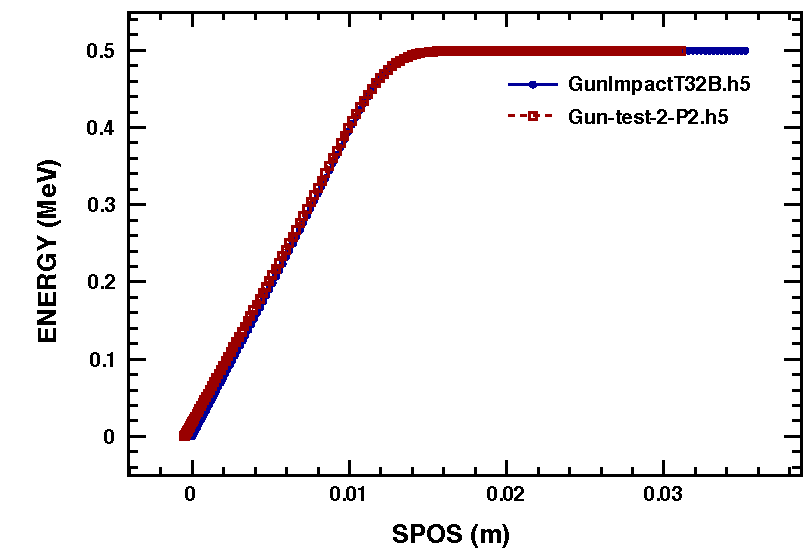
\includegraphics[width=0.6\linewidth,angle=90]{figures/Gun/GunCompEn}
%   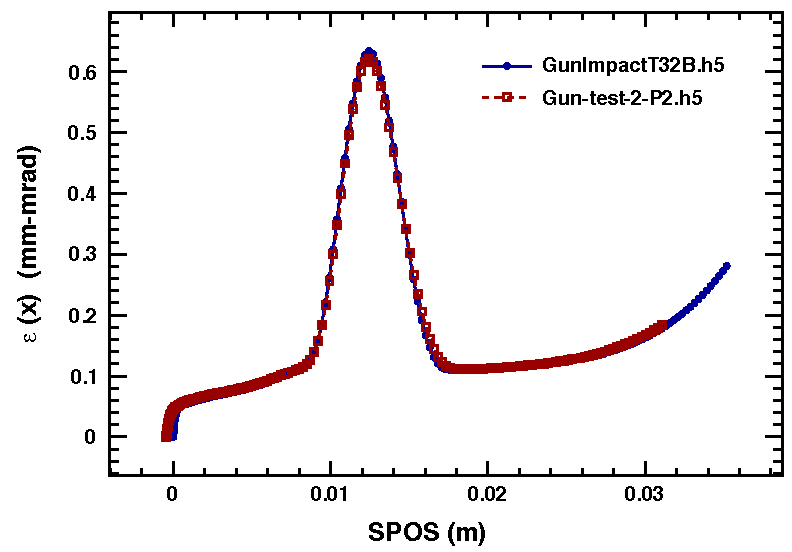
\includegraphics[width=0.6\linewidth,angle=90]{figures/Gun/GunCompEx}
%   \caption{Comparison of energy and emittance in $x$ between \impactt and \opalt}
%   \label{fig:guncomp2}
% \end{center}
%\end{figure}

\subsection{PSI XFEL 250 MeV Injector}
\label{sec:felinj}
\index{XFEL}
\index{INJECTOR}
\examplefromfile{examples/diagnostic.in}



\subsection{PSI Injector II Cyclotron}
\label{sec:inj2}
\index{INJECTOR II}
\index{CYCLOTRON}
%%%%%%%%%%
Injector II is a separated sector cyclotron specially designed for pre-acceleration (inject: \SI{870}{\kilo\electronvolt}, extract: \SI{72}{\mega\electronvolt} )
of high intensity proton beam for Ring cyclotron. It has 4 sector magnets, two double-gap acceleration cavities
(represented by 2 single-gap cavities here) and two single-gap flat-top cavities.

Following is an input file of {\bfseries Single Particle Tracking mode} for PSI Injector II cyclotron.

\examplefromfile{examples/opal-cycl.in}

To run opal on a single node, just use this command:
\begin{example}
 opal testinj2-1.in
\end{example}

Here shows some pictures using the resulting data from single particle tracking using \opalcycl.

Left plot of \figref{Inj2 reference orbit and tune} shows the accelerating orbit of reference particle. After 106 turns, the energy increases from \SI{870}{\kilo\electronvolt} at the injection point to \SI{72.16}{\mega\electronvolt} at the deflection point.

%======================FIGURE===============================
\begin{figure}[tb]
\centering
   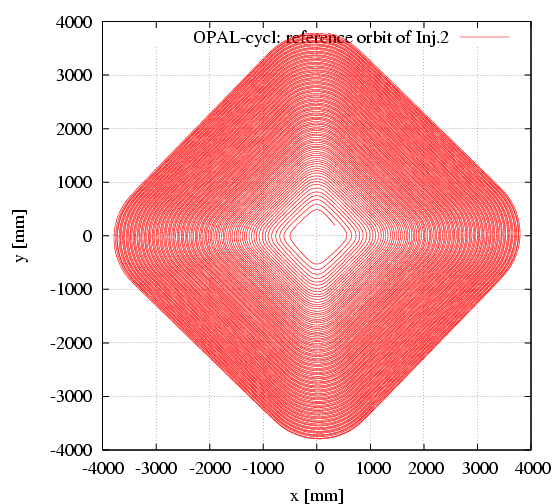
\includegraphics[width=0.45\textwidth]{figures/cyclotron/AEO_Injector2.png}
   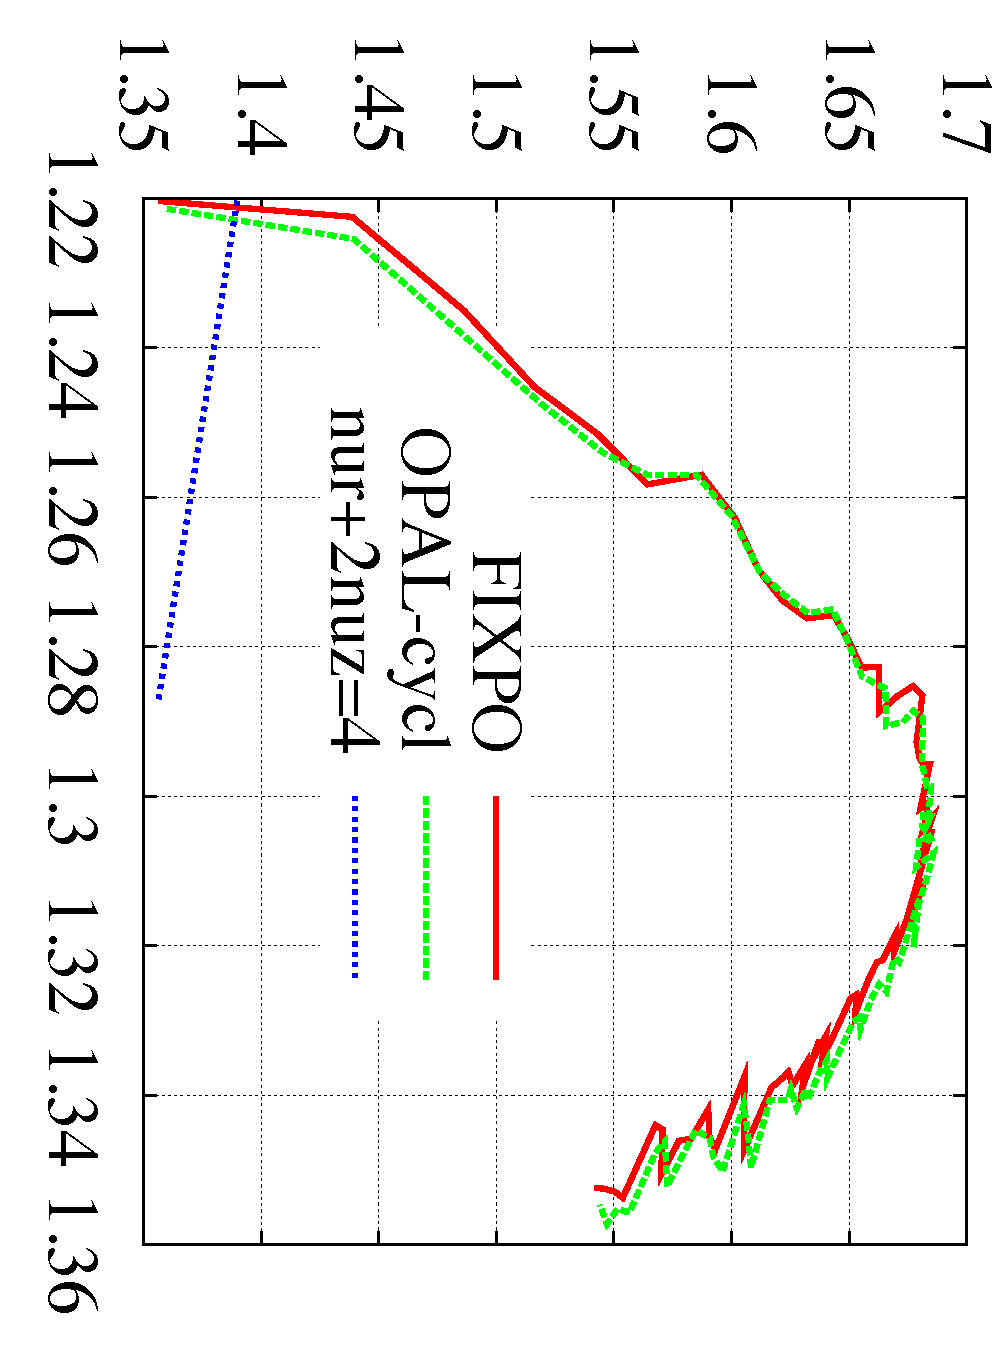
\includegraphics[width=0.40\textwidth,angle=90]{figures/cyclotron/nurnuz_Inj2}
   \caption{Reference orbit(left) and tune diagram(right) in Injector II  }
   \label{fig:Inj2 reference orbit and tune}
\end{figure}
%===========================================================


From theoretic view, there should be an eigen ellipse for any given energy in stable area of a fixed accelerator structure. Only when the initial phase space
shape matches its eigen ellipse, the oscillation of beam envelop amplitude will get minimal and the transmission efficiency get maximal.
We can calculate the eigen ellipse by single particle tracking using betatron oscillation property of off-centered particle as following: track
an off-centered particle and record its coordinates and momenta at the same azimuthal position for each revolution.
\figref{eigen} shows the eigen ellipse at symmetric line of sector magnet for energy of \SI{2}{\mega\electronvolt} in Injector II.

%======================FIGURE===============================
\begin{figure}[tb]
\centering
   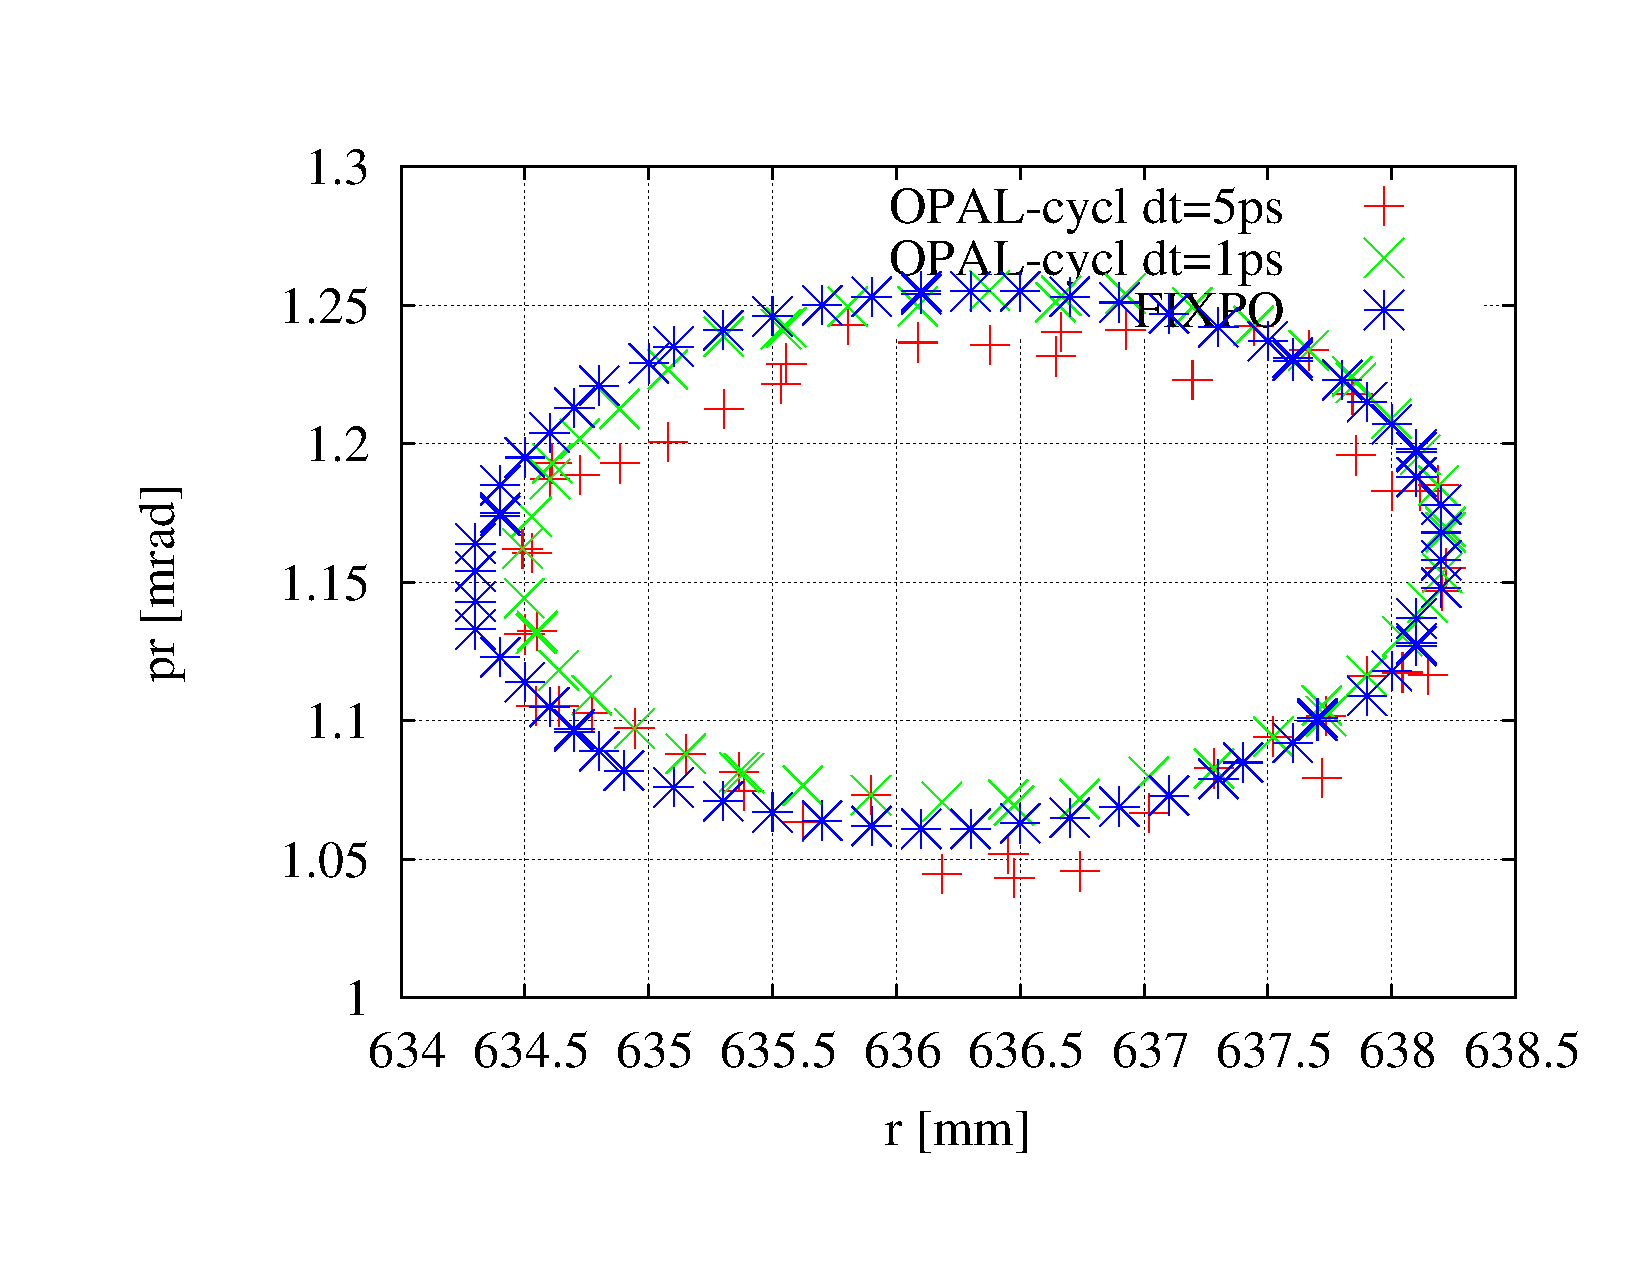
\includegraphics[width=0.45\textwidth]{figures/cyclotron/RadialEigen_Inj2}
   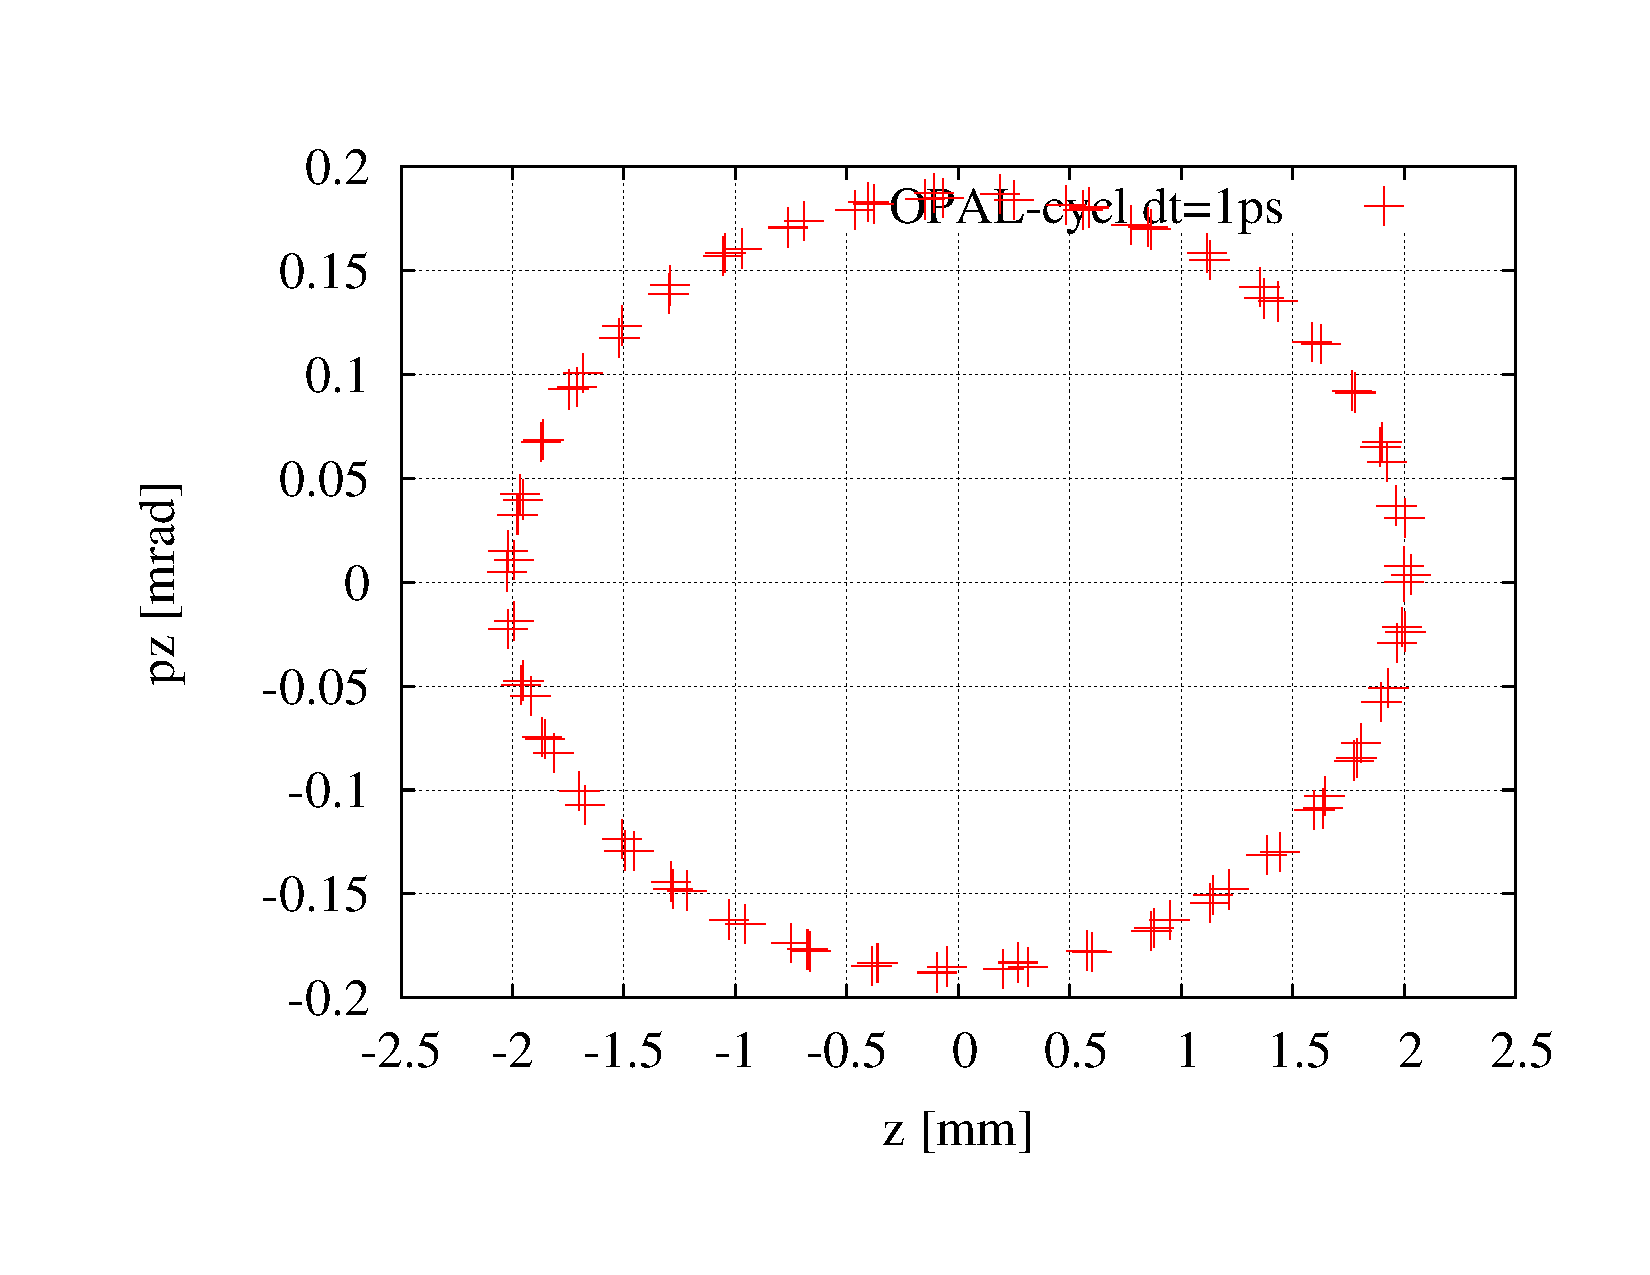
\includegraphics[width=0.45\textwidth]{figures/cyclotron/VertEigen_Inj2}
   \caption{Radial and vertical eigenellipse at \SI{2}{\mega\electronvolt} of Injector II}
   \label{fig:eigen}
\end{figure}
%===========================================================


Right plot of \figref{Inj2 reference orbit and tune} shows very good agreement of the tune diagram by \opalcycl and FIXPO.
The trivial discrepancy should come from the methods they used.
In FIXPO, the tune values are obtained according to the crossing points of the initially displaced particle. Meanwhile, in \opalcycl, the Fourier
analysis method is used to manipulate orbit difference between the reference particle and an initially displaced particle.
The frequency point with the biggest amplitude is the betatron tune value at the given energy.

%%%%%%%%%%%%%%
Following is the input file for single bunch tracking with space charge effects in Injector II.
%%%%%%%%%%%%%%

\examplefromfile{examples/opal-cycl-sc.in}

To run opal on single node, just use this command:
\begin{example}
 # opal testinj2-2.in
\end{example}

To run opal on N nodes in parallel environment interactively, use this command instead:
\begin{example}
 # mpirun -np N opal testinj2-2.in
\end{example}

If restart a job from the last step of an existing \filename{.h5} file, add a new argument like this:
\begin{example}
 # mpirun -np N opal testinj2-2.in -restart -1
\end{example}
\figref{cyclParameters,cyclphasespace} are simulation results, shown by  H5ROOT code.

%======================FIGURE===============================
\begin{figure}[tb]
\centering
    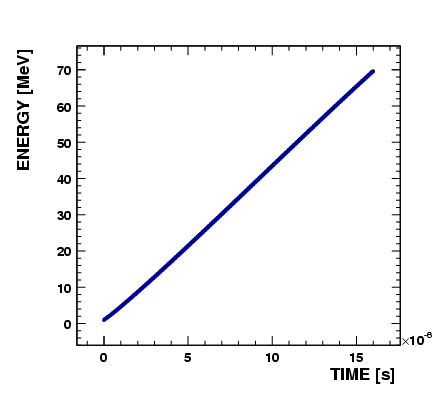
\includegraphics[width=0.45\textwidth]{figures/cyclotron/Inj2-ENERGY-TIME.png}
    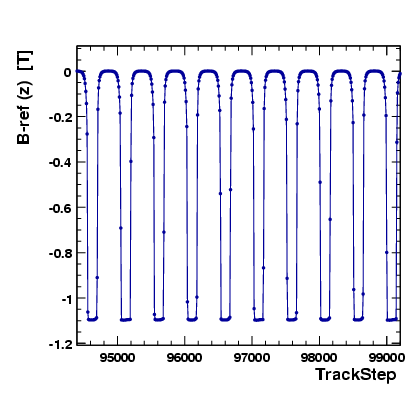
\includegraphics[width=0.45\textwidth]{figures/cyclotron/Inj2-B-ref-z-TrackStep.png}
    \caption{Energy Vs. time (left) and external B field Vs. track step (Right, only show for about 2 turns)}
    \label{fig:cyclParameters}
\end{figure}
%===========================================================


%======================FIGURE===============================
\begin{figure}[tb]
\centering
    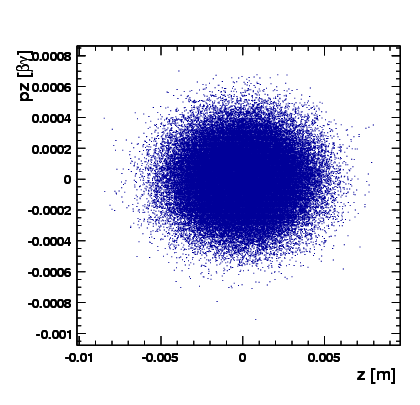
\includegraphics[width=0.3\textwidth]{figures/cyclotron/Inj2-z-pz-step-870KeV.png}
    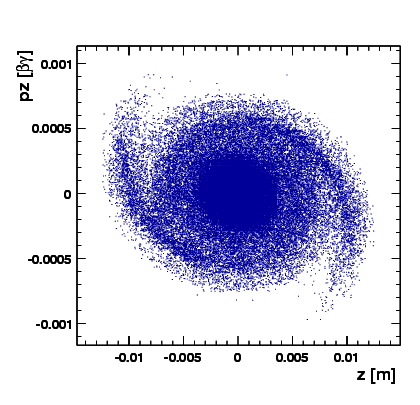
\includegraphics[width=0.3\textwidth]{figures/cyclotron/Inj2-z-pz-step-15MeV.png}
    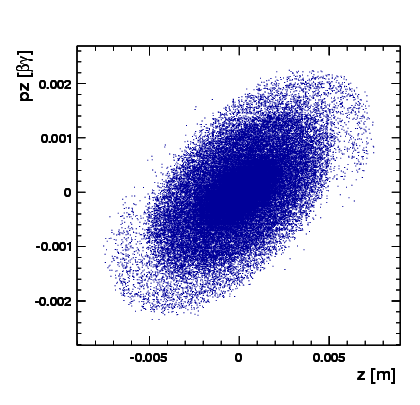
\includegraphics[width=0.3\textwidth]{figures/cyclotron/Inj2-z-pz-step-30MeV.png}
    \caption{Vertical phase at different energy from left to right: \SI{0.87}{\mega\electronvolt}, \SI{15}{\mega\electronvolt} and \SI{35}{\mega\electronvolt}}
    \label{fig:cyclphasespace}
\end{figure}
%===========================================================



%%%%%%%%%%%%%%
\subsection{PSI Ring Cyclotron}
\label{sec:Ring}
\index{RING}
\index{CYCLOTRON}
From the view of numerical simulation, the difference between Injector II and Ring cyclotron comes from two aspects:
\begin{description}
\item[B Field] The structure of Ring is totally symmetric, the field on median plain is periodic
along azimuthal direction, \opalcycl take this advantage to only store \nicefrac{1}{8} field data to save memory.

\item[RF Cavity] In the Ring, all the cavities are typically single gap with some parallel displacement from its
radial position.\opalcycl have an argument \keyword{PDIS} to manipulate this issue.
\end{description}
\begin{figure}[ht]
  \begin{center}
    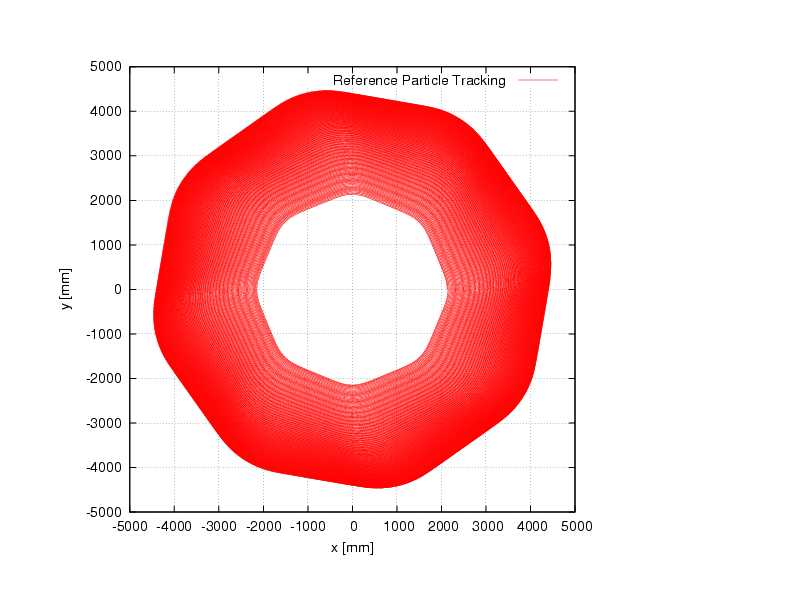
\includegraphics[width=6cm,trim=2.5cm 2.5cm 2.5cm 2.5cm]{figures/cyclotron/AEO_Ring.png}
    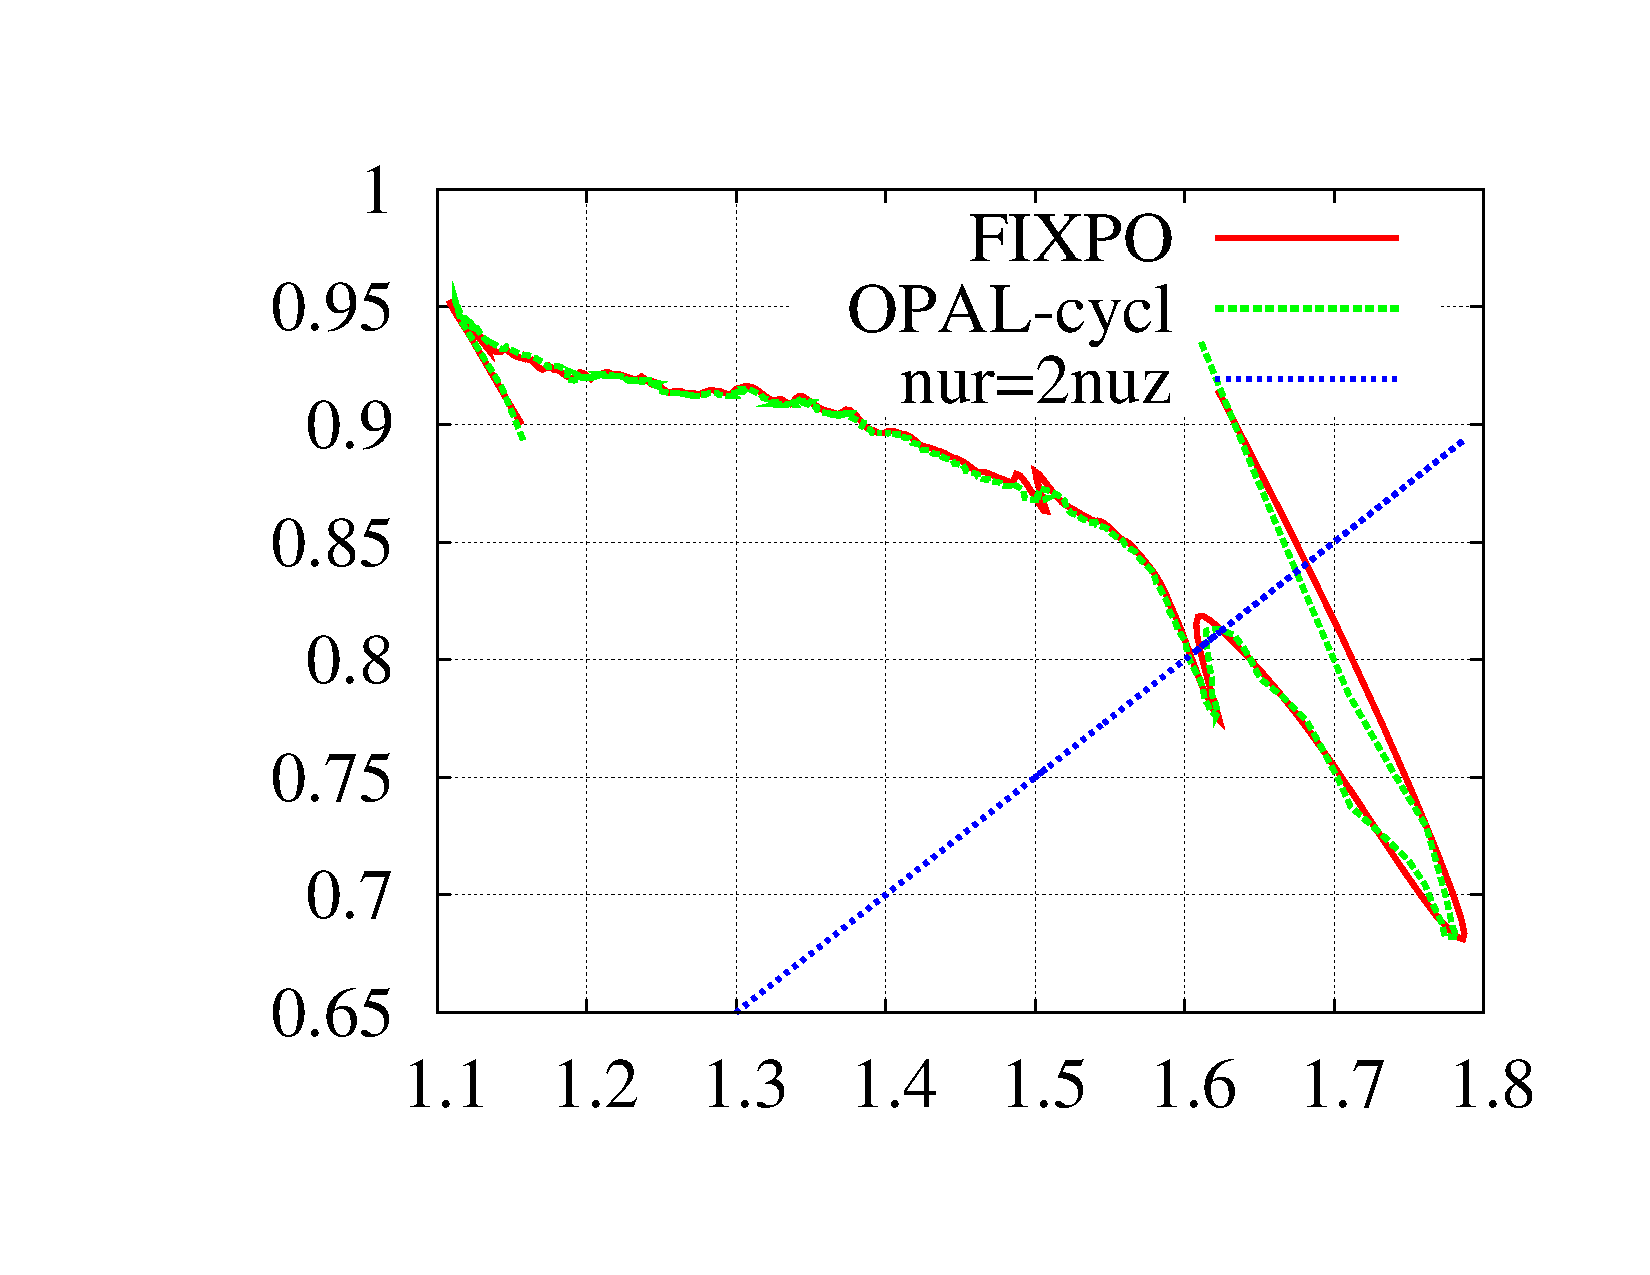
\includegraphics[width=6cm,trim=2.5cm 2.5cm 2.5cm 2.5cm]{figures/cyclotron/nurnuz_Ring}
    \caption{Reference orbit(left) and tune diagram(right) in Ring cyclotron }
    \label{fig:Ring reference orbit and tune}
  \end{center}
\end{figure}
\figref{Ring reference orbit and tune} shows a single particle tracking result and tune calculation result in the PSI Ring cyclotron.
Limited by size of the user guide, we don't plan to show too much details as in Injector II.

\clearpage


\section{Translate Old to New Distribution Commands}
\label{sec:oldtonewdist}
\index{Distribution!Translate Old}
As of \opal 1.2, the distribution command \seechp{distribution} was changed significantly. Many of the changes were internal to the code, allowing us to more easily add new distribution command options. However, other changes were made to make creating a distribution easier, clearer and so that the command attributes were more consistent across distribution types. Therefore, we encourage our users to refer to \chpref{distribution} when creating any new input files, or if they wish to update existing input files.

With the new distribution command, we did attempt as much as possible to make it backward compatible so that existing \opal input files would still work the same as before, or with small modifications. In this section of the manual, we will give several examples of distribution commands that will still work as before, even though they have antiquated command attributes. We will also provide examples of commonly used distribution commands that need small modifications to work as they did before.

\textbf{\emph{An important point to note is that it is very likely you will see small changes in your simulation even when the new distribution command is nominally generating particles in exactly the same way.}} This is because random number generators and their seeds will likely not be the same as before. These changes are only due to \opal using a different sequence of numbers to create your distribution, and not because of errors in the calculation. (Or at least we hope not.)

\subsection{\keywordinheader{GUNGAUSSFLATTOPTH} and \keywordinheader{ASTRAFLATTOPTH} Distribution Types}
\label{sec:oldtonewdistgungaussandastra}
\index{Distribution!Translate GUNGAUSSFLATTOPTH}
\index{Distribution!Translate ASTRAFLATTOPTH}
The \keyword{GUNGAUSSFLATTOPTH} and \keyword{ASTRAFLATTOPTH} distribution types \seesec{gungaussflattopthdisttype,astraflattopthdisttype} are two common types previously implemented to simulate electron beams emitted from photocathodes in an electron photoinjector. These are no longer explicitly supported and are instead now defined as specialized sub-types of the distribution type \keyword{FLATTOP}. That is, the \emph{emitted} distributions represented by \keyword{GUNGAUSSFLATTOPTH} and \keyword{ASTRAFLATTOPTH} can now be easily reproduced by using the \keyword{FLATTOP} distribution type and we would encourage use of the new command structure.

Having said this, however, old input files that use the \keyword{GUNGAUSSFLATTOPTH} and \keyword{ASTRAFLATTOPTH} distribution types will still work as before, with the following exception. Previously, \opal had a Boolean \keyword{OPTION} command \keyword{FINEEMISSION} (default value was \keyword{TRUE}). This \keyword{OPTION} is no longer supported. Instead you will need to set the distribution attribute \keyword{EMISSIONSTEPS} \seetab{distattremitted} to a value that is 10 $\times$ the value of the distribution attribute \keyword{NBIN} \seetab{distattruniversal} in order for your simulation to behave the same as before.
%----------- Footer control ------------------
\ifthenelse{\boolean{FullOPALManual}}
{
  %do nothing
}
% else (for individual document creation)
{
\appendix
\printbibliography
\end{document}
}
%---------------------------------------------

\subsection{\keywordinheader{FROMFILE}, \keywordinheader{GAUSS} and \keywordinheader{BINOMIAL} Distribution Types}
\index{Distribution!Translate FROMFILE}
\index{Distribution!Translate GAUSS}
\index{Distribution!Translate BINOMIAL}
The \keyword{FROMFILE} \seesec{fromfiledisttype}, \keyword{GAUSS} \seesec{gaussdisttype} and \keyword{BINOMIAL} \seesec{binomialdisttype} distribution types have changed from previous versions of \opal. However, legacy distribution commands should work as before with one exception. If you are using \opalcycl then your old input files will work just fine. However, if you are using \opalt then you will need to set the distribution attribute \keyword{INPUTMOUNITS} \seesec{unitsdistattributes} to:
\begin{example}
INPUTMOUNITS = EV
\end{example}